\documentclass{IEEEtran}
\usepackage{graphicx}
\addcontentsline{toc}{chapter}{Bibliography}
\usepackage{amsmath}
\usepackage{amssymb}
\usepackage{algorithm}
\usepackage[noend]{algpseudocode}

\begin{document}


\title{Resource Allocation by Diversity}
\author{Yuri Lavinas}

\maketitle



\begin{abstract}
	
	Multi-objective Evolutionary Algorithm based on Decomposition decomposes a multi-objective problem into simpler, single-objective subproblems by means of scalarizations. In it, all subproblems are uniformly treated, i.e, there is no priority among them. Each subproblem is related to a area of the theoretical Pareto Front, and it is expected that different areas would be more difficult to find approximations that other areas. Therefore, this may lead to an unbalanced exploration of the search space. In this work the goal is to analyze a prioritizing function based on an on-line diversity metric. hence, we perform an experimental study of the proposed algorithm, with NSGA-2, MOEA/D-DE and MOEA/D-GRA on both benchmark group functions, the WFG and the recently proposed bbob-biobj. The results indicate that XXX.
\end{abstract}

\section{Introduction}

Multi-objective Optimization Problems (MOPs)~\cite{miettinen1999nonlinear} are problems composed of two or more functions which must be simultaneously optimized by the same set of parameters. This composition is characterized by a set of conflicting objective functions resulting in a set of optimal compromise solutions. 

These $m$ multiple objective functions must be optimized simultaneously:

\begin{align}\label{min_problem}
\text{minimize} f(x) = (f_1(x), ..., f_{m}(x)), \text{ with $x \in \mathbb{R}^{D}$},
\end{align}

where $m$ is the number of objective functions and $\mathbb{R}^m$ is the objective function space. $x \in \mathbb{R}^{D} = \{x_1, x_2, ..., x_D\}$ is a D-dimensional vector and it represents a candidate solution with ${D}$ variables, $f: \mathbb{R}^{D} \rightarrow \mathbb{R}^{m}$ is a vector of objective functions.% and $\Omega$ is the feasible decision space. $\Omega$ is defined as:

%\begin{align}
%\Omega =\{x \text{ in } \mathbb{R}^{n_v} | g_i(x) \leq 0 \text{ } \forall_i \text{ and } h_i(x) = 0 \text{ } \forall_j \},
%\end{align}
These objectives often conflict with each other, as there is no point in $\mathbb{R}^{D}$ that minimizes all the objectives at the same time. Consequently, the goal of the MOP optimization algorithm is to find the approximate sets of solutions that balance the different objectives in an optimal way.

Given two solutions vectors $u, v$ in $\mathbb{R}^{D}$, $u$  Pareto-dominates $v$, denoted by $f(u) \prec f(v)$, if and only if $f_k(u) \leq f_k(v), \forall_k \in \{1,..., m\}$ and $ f(u) \neq f(v)$. Likewise, a solution $x \in \mathbb{R}^{D}$ is considered Pareto-Optimal if there exists no other solution $y \in \mathbb{R}^{D}$ such that $f(y) \succ f(x)$, i.e., if $x$ is non-dominated in the feasible decision space. A non-dominated solution exists if no other solution provides a better balance in all objectives.

Consequently, the set of all Pareto-Optimal solutions is known as the Pareto-Optimal Set (PS), while the image of this set is referred to as the Pareto-optimal Front (PF).\\

\begin{equation}
PS = \{x \in \mathbb{R}^{D} | \nexists y \in \mathbb{R}^{D} : f(y) \succ f(x)  \},
\end{equation}

\begin{equation}
PF = \{f(x) | x \in PS \}.
\end{equation}

Multi-objective evolutionary algorithms (MOEAs) are one of the most widely used groups of algorithms for finding approximations to the PF of a MOP. They are characterized by their ability to find good approximations to PF in a single run~\cite{zhou2011multiobjective}. In recent years, there has been an increasing interest in studying MOEAs and with a primary concern of improving their general performance. Among MOEAs, there are three major paradigms: Pareto domination-based approaches~\cite{deb2002fast},~\cite{zitzler2001spea2}; the indicator-based approaches~\cite{beume2007sms},~\cite{zitzler2004indicator} and the decomposition-based approaches~\cite{li2009multiobjective},~\cite{zhang2007moea}. 

In this study, we are interested in analyzing the Multi-objective Evolutionary Algorithm based on Decomposition framework, MOEA/D~\cite{zhang2007moea}. It represents a class of population-based meta-heuristics for solving Multi Objective Problems~\cite{trivedi2017survey}. In this framework, the original multi-objective problem is decomposed into simpler, single-objective subproblems by means of scalarizations which defines the weights vectors. Each subproblem is then evaluated and its utility value is calculated by an aggregation function given the related weight vector. In the original MOEA/D, all the subproblems have the same amount of computational resource (number of iteractions). 
%\begin{figure}[h]
%	\centering
%	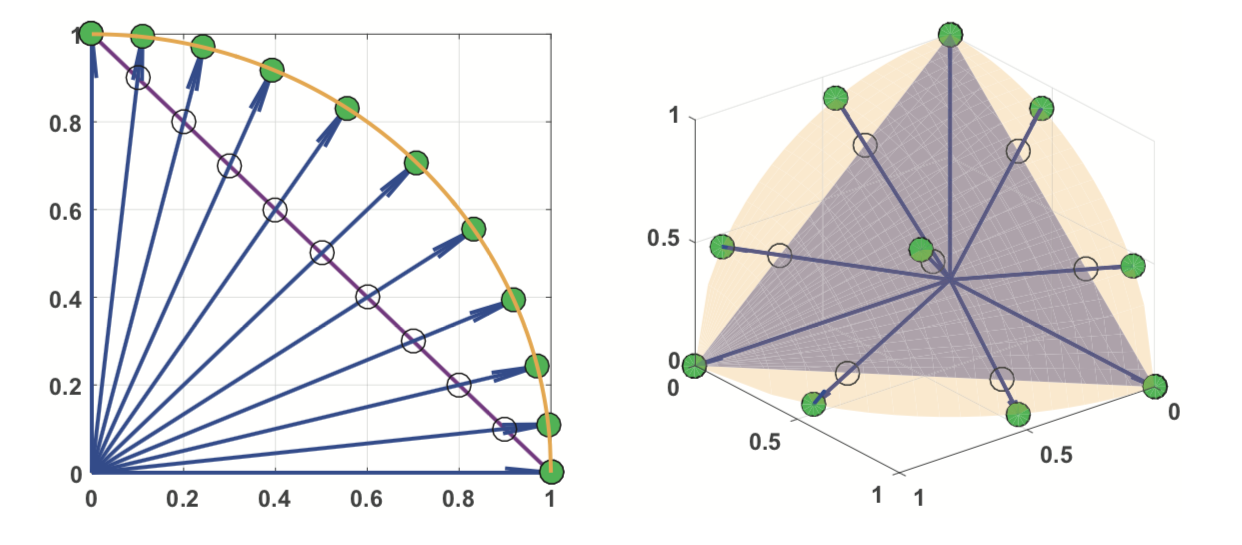
\includegraphics[width=0.55\textwidth]{img/decomp2.png}
%	\caption{A decomposition strategy generates weight vectors that defines the subproblems. Figure from~\cite{chugh2017handling}.}
%	\label{fig1}
%\end{figure}
%
%\begin{figure}[h]
%	\centering
%	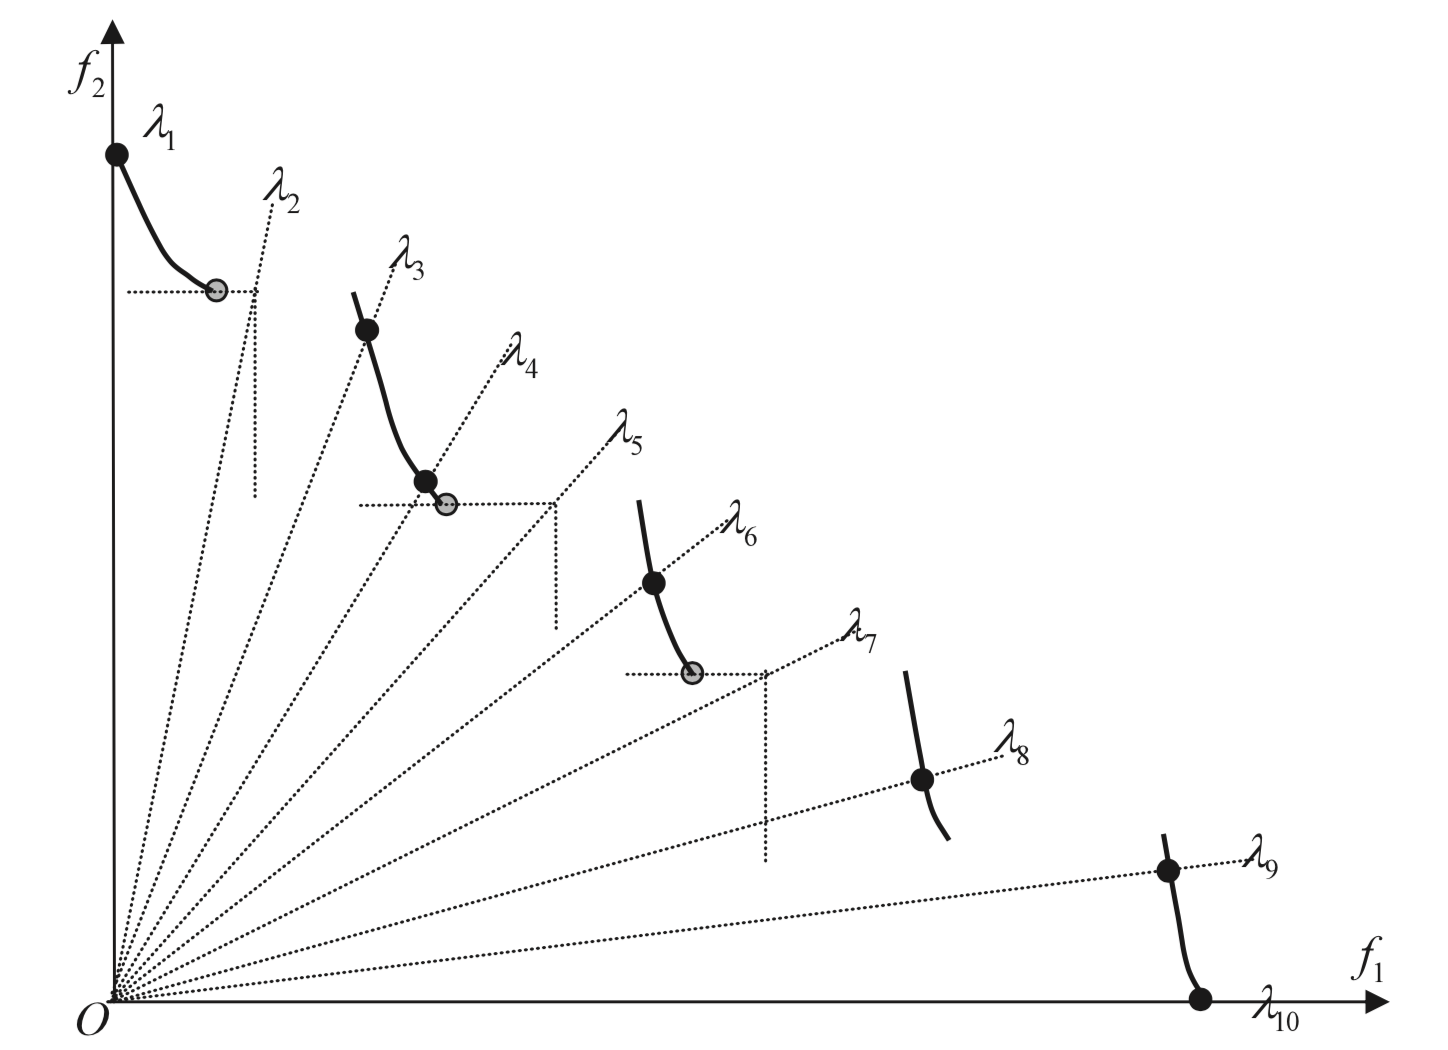
\includegraphics[width=0.43\textwidth]{img/harder_problems}
%	\caption{Distribution of optimal solutions of subproblems with uniform weight vectors on ZDT3. Figure from~\cite{li2015use}.}
%	\label{fig2}
%\end{figure}
%
%
%\begin{figure}[h]
%	\centering
%	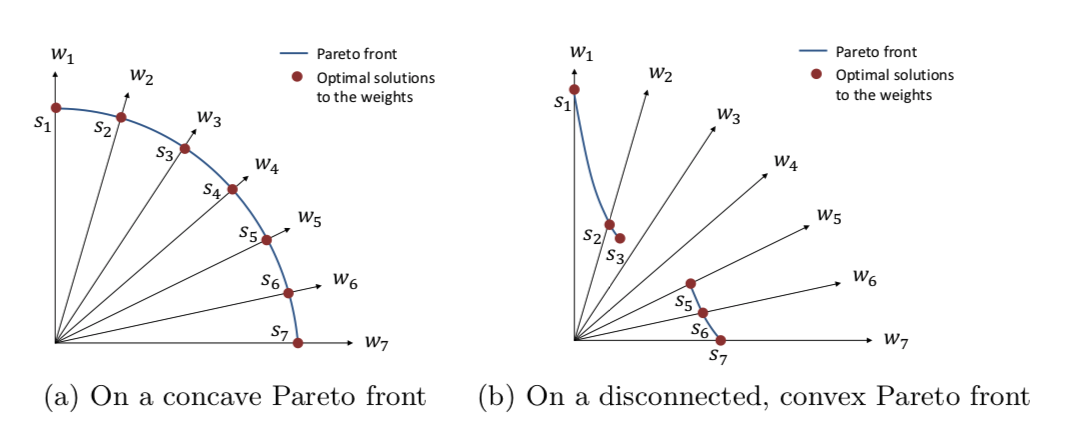
\includegraphics[width=0.53\textwidth]{img/harder_problems2}
%	\caption{An example that uniformly distributed weights may lead to different distributions of optimal solutions. (a) Solutions $s_1$ to $s_7$ are the optimal solutions of weights $w_1$ to $w_7$, respectively. (b) Solutions $s_1$,$s_2$,$s_3$,$s_6$ and $s_7$ are the optimal solutions of $w_1$,$w_2$,$w_3$,$w_6$ and $w_7$, respectively, while solution $s_5$ is the optimal solution of $w_4$ and $w_5$.Figure from~\cite{li2017weights}}
%	\label{fig3}
%\end{figure}



%It represents a class of population-based meta-heuristics for solving MOPs. Many other algorithms exists as NSGA-2(3), MOEA/Ds, IBEA, SPEA2, DEMO.
%interest of the PF. This duality between regions may lead to an unbalanced exploration of the search space, since it would be preferable to focus only on subproblems related to regions of interest.

Although researchers have not studied this problem in much detail, there have been some works that have discussed this matter. One way to address this problem is to adjust the behavior of the algorithm in an online manner to suit the problem in question~\cite{hinterding1997adaptation},~\cite{de2007parameter},~\cite{meyer2007self},~\cite{zhang2009performance},~\cite{kramer2010evolutionary},~\cite{zhang2012survey}~\cite{cai2015external}. All algorithmic components can be tunned adaptively and often feedback information is needed for these adaptation strategies. 

Another way, is  allocating different number of evaluations to the subproblems based on some priority function. In a few recent works, a utility function is used to prioritize resources given to subproblems that contribute more to the algorithm's search.  In the works of Zhang et al.~\cite{zhang2009performance} and Zhou et al.~\cite{zhou2016all} a utility function was proposed aiming to prioritize solutions based on a historical convergence information during different generations. Another approach was implemented in~\cite{kang2018collaborative}, where the utility function was based on the presence of a solution from the main population on a secondary population.

The aim of this study is to explore the relationship between subproblems and utility functions. Here, we propose a new methodology for defining these priority functions given a diversity metric. This studies examines the integration of an online diversity metric based on a geometrical perspective~\cite{gee2015online} as direct way to define the utility function. Unfortunately, a full discussion of diversity metrics as utility function lies beyond the scope of this study.
%The main contributions of this paper can be summarized as follows:

%\begin{itemize}
%	\item blablabla
%	\item blebleble
%	\item bliblibli
%\end{itemize}

%This work is divided in sections and subsections according to this and that.


\section{Related Works}

\subsection{Utility functions}

%Following the discussion opened in the introduction, we need to define an utility function to allocate the number of evaluations to subproblems. 

Utility functions monitor the algorithm performance and may be used to decide how to distribute the computation resources among subproblems, guiding the search behavior of the algorithm. They are one way of defining priorities~\cite{chankong1983multiobjective},\cite{hansson2005decision},  and may be used as one way of deciding computational resources distributions among subproblems by guiding the distribution over generations~\cite{cai2015external}. 


To the best of the authors knowledge, there is a relatively small body of the literature concerned with resource allocation. Few previous studies are listed here: MOEA/D-DRA~\cite{zhang2009performance}; MOEA/D-GRA~\cite{zhou2016all}; and MOEA/D-AMS~\cite{chiang2011moea}. On most of them, there is moderated justification for the reason of why the utility function is defined. Also, limited explanation of why these functions help the MOEA/D search.

According to Zhou and Zhang~\cite{zhou2016all}, MOEA/D-GRA may be seen as an generalization of MOEA/D-DRA and MOEA/D-AMS. The reason is that all of these algorithm use a very similar utility function. In all, the utility function, $u = \{u_1, u_2, ..., u_N\}$ for every subproblem $i=1,...,N$, is as defined in the next equation.

\begin{equation}\label{utility}
	u_i = \dfrac{\text{old fun val}-\text{new fun val}}{\text{old fun val}}.
\end{equation}


The idea that supports this equation is that if a subproblem has been improved over the last $\Delta T$ generations (\textit{old function value}), it should have a high probability to be improved over the next few generations. 

In contrast, the utility function used in MOEA/D-CRA~\cite{kang2018collaborative}, is based on if of an individual from population $A$ is selected to compose the population $B$. This MOEA/D variation is based on the MOEA/D-M2M~\cite{liu2014decomposition}, a variation with two populations. 

Together these studies indicate that it is worth monitoring the algorithm behavior and guiding its search, but it is unclear if the utility functions proposed are the most appropriated ones. Besides it remains vague how these functions affect the algorithm results.

Consequently, in this work, we propose to define an utility function supported by a diversity metric based on a geometrical interpretation of convergence and diversity. This new function is then integrated to MOEA/D-GRA. The benefit of using MOEA/D-GRA as based is that it has a straightforward implementation, it achieved good overall results in the experimental analysis of Zhou and Zhang~\cite{zhou2016all}  and it is a good representative of a the class of variants of MOEA/D with resource allocation.

\subsection{Diversity Metric}

Some works in diversity metrics over the last 2 decades have successfully  proposed and applied in different task on evolutionary computation. 



%Here, I use MRDL as a way to assess the diversity of solutions in an on-line manner and use a utility function based on the output of this metric to guide resource allocation at each generation. 

One way to measure diversity is to use metrics that evaluate MOPs solvers that consider diversity. The hyper-volume indicator (HV)~\cite{zitzler1998multiobjective} and the Inverted Generational Distance (IGD)~\cite{zhang2008rm} are frequently used as metrics to evaluate such solvers. However they include information about both convergence and diversity in a single metric.

Among the metrics that only measure diversity, there are mainly two groups. The first one is the offline group, that calculate the diversity after the execution of the algorithm, and the second is the online group, that calculate the diversity during the execution of the algorithm. Following some studies that are part of these groups are briefly introduced. Both lists are not extensive ones.

 The offline group is composed off: Chi-square-like deviation~\cite{deb1989genetic}; Spacing method~\cite{scott1995fault}; Uniformly distribution index~\cite{tan2002evolutionary}; Entropy approach~\cite{farhang2002diversity}; Grid diversity metric~\cite{deb2002running}; sparsity measure~\cite{deb2003fast}. These published studies need knowledge of the PF or the ideal vector. While the online group is composed off sigma method~\cite{mostaghim2003strategies}  (PF lies in the positive objective space); entropy of the solutions by using Parzen window density estimation-\cite{tan2008evolutionary} (sensitive to kernel width); maximum relative diversity loss~\cite{gee2015online} (expensive $O(N^2)$, with $N$ being the size of the parent population).

In this work the maximum relative diversity loss was chosen to an online diversity assessment to measure the diversity loss caused by any individual in the population and then guide the resource allocation at each generation. Since it is a very costly metric, in future works other metrics are going to be analyzed.




\section{Proposed Method}

MOEA/D-RAD, MOEA/D with on-line Resource Allocation by Diversity Metric, is the variant of MOEA/D proposed in this work. This algorithm uses the maximum relative diversity loss, MRDL, for determining the values of the utility function. 

\begin{algorithm}[h]
	\caption{MOEA/D-RAD}\label{alg1}
	\begin{algorithmic}[1]

	\State Initialize the weight vectors $\lambda_i$, the neighborhood $B_i$, the utility value $u_i$ every subproblem $i=1,...,N$.
		
		\While{\textit{Termination criteria}}
		\For {1 to N}
			\If{$\textit{rand()} < u_i$}\Comment{From MOEA/D-GRA}
				\State Generate a offspring $y$ for subproblem $i$.
				\State Update the population by $y$.
			\EndIf
	\EndFor
	\State Update \textit{\textbf{u}} by a diversity metric after $\Delta T$ generations.
		\EndWhile
	\end{algorithmic}
\end{algorithm}


The algorithm~\ref{alg1} describe MOEA/D-RAD. Except from line 4, in which a subproblem may not be part of the group that is going to be iterated and from line 7, in which the utility function is calculated, the whole procedure is similar to the MOEA/D-DE~\cite{zhang2009performance}. Likewise, all reproduction procedures and parameters are the same as in MOEA/D-DE~\cite{li2009multiobjective}. It is important to highlight that the neighborhood is only calculated in the initialization period.

%The update procedure is described The algorithm~\ref{alg2}, as in MOEA/D-GRA~\cite{zhou2016all}.
The decomposition method used is the Simple-Lattice Design (SLD), the scalar aggregation function Weighted Sum (WS), the Restricted update strategy.

We initialize the value of the vector $u=1$, as in MOEA/D-DRA. As in MOEA/D-DRA and GRA we have a learning period, $\Delta T$ generations (\textit{old function value}). Here, the $\Delta T=20$.   A sensitivity analyzes need to be performed for deciding suitable initial values for $u$ for $\Delta T$.

\subsection{Utility Function by Diversity} 

%\begin{figure}[!t]
%	\centering
%	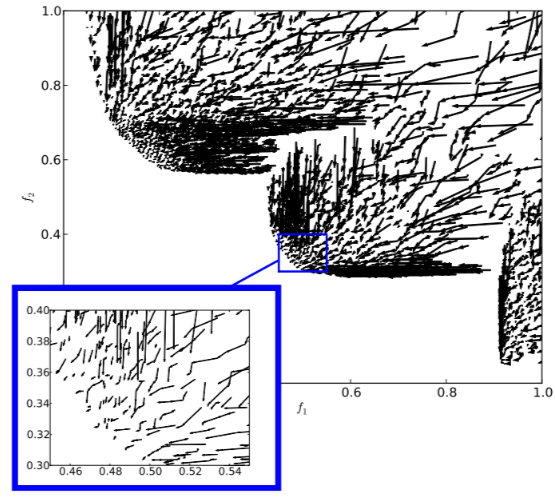
\includegraphics[width=0.47\textwidth]{img/conv_dir}
%	\caption{Estimated convergence directions over 500 generations in CEC-09 UF1 benchmark test problem.Figure from~\cite{gee2015online}}
%	\label{fig4}
%\end{figure}

The utility function proposed in this work is based on the Maximum Relative Diversity Loss MRDL. Prior to scalarizing it between $0$ and $1$ to fit the algorithm~\ref{alg1} we calculate MRDL for every individual of the population. The following function describes how to calculate the utility function given the MRDL, $\Gamma^{p \rightarrow c}$, as follows.

\begin{equation}
u_i = \Gamma^{p \rightarrow c}_i -  \Gamma^{p \rightarrow c}_j, \text{with  $i=1,...,N$.}
\end{equation}

%For the purpose of defining the utility function used in this work, we need to define the MRDL.

MRDL is an online diversity metric that estimates the diversity loss of a solution to the whole population~\cite{gee2015online}. First, it is an useful metric since if a new offspring generated is identical to any offspring solution in the convergence archive, the metric value will be infinite. Second, high values of  indicates the existence of similar offspring solution in the convergence archive or the offspring solution is close to the line of estimated convergence direction. Finally, it may be used as an adaptive technique to adjust parameters, as applied in its original study~\cite{gee2015online}.

The idea of the MRDL is to use the space movement (convergence directions) of a solution on the objective space towards the PF. The further an objective vector of a solution is from the convergence direction, more it contributes for the diversity of the approximated PF.

%This is done since the convergence direction is perpendicular to the diverse direction. Here we use the definition of convergence as solutions approaching to the POF in the objective space for the first, while for diversity as the spreading and distribution of solutions along the PF~\cite{gee2015online}.

To compute the MRDL, we need to estimate $k$ convergence directions at every generation. Then we need to  approximate the Relative Diversity Loss (RDL) for each of these $k$ convergence directions. To calculate this estimative of diversity loss of a solution to the whole population, the following equation is used, considering every incumbent solution related to a subproblem $i$, from the whole population.
 

\begin{equation}
\Gamma_{i}^{p \rightarrow c} = \underset{i=1,...,k}{\max} \Gamma_{d.conv_{y}}^{p \rightarrow c},
\end{equation}




RDL is a diversity measurement quantity that indicates the amount of diversity loss of an individual solution between two consecutive generations. High values of RDL imply a reduction of the solution spread and this equation may indicated the amount of diversity loss.

This quantity is given by a division between the shortest distance of a parent, $p$,  and offspring, $c$, to the line of convergence direction.

\begin{equation}
\label{rdl}
\Gamma_{d.conv_{y}}^{p \rightarrow c} = \dfrac{ ||p \prime - proj_{d.conv_{y}}p \prime|| }{||c \prime - proj_{d.conv_{y}}c \prime||}
\end{equation}

The numerator in~\ref{rdl} is the closest distance between the parent solution ($p$) to the convergence direction $(c_r - p_r)$. While, the denominator in~\ref{rdl} is the closest distance between the offspring solution ($c$) to the convergence direction $(c_r - p_r)$. %The projections of $p\prime$ and $c\prime$ objective vectors onto the convergence direction $d.conv_{y}$ are $proj_{d.conv_{y}}p \prime$ and $proj_{d.conv_{y}}c \prime$.

with $p\prime$ and $c\prime $ given by:

\begin{equation}
\begin{split}
p\prime = p - p_r,\\
c\prime = c - c_s,\\
\end{split}
\end{equation}
%verify this

with $p_r$ and $c_s$ being the parent and offspring objective vectors used to calculate the convergence direction in equation~\ref{1}. That is the index $s$ is equal to the index $j$ used to calculate $conv_{y}$. The same principle is valid for the index $r$.
 
The vector projection between two vectors is defined as next.

\begin{equation}
proj_{d.conv_{y}}p \prime = \frac {{d.conv_{y}} \cdot {p \prime}} {|{p \prime}|^2}{{p \prime}}.
\end{equation}

While the norm of $p \prime - proj_{d.conv_{y}}p \prime$ is calculated as follows.


\begin{equation}
||p \prime - proj_{d.conv_{y}}p \prime|| = sqrt(crossprod(proj_{d.conv_{y}}p \prime))
\end{equation}

and the norm of $c \prime - proj_{d.conv_{y}}c \prime$ is calculated similarly.


To estimate the convergence direction, $d.conv_{y}$, we need to have a offspring, $c_j$, that dominates a parent. Select a parent, $p_h$, solution that is closest to this offspring in the objective space. 

For every weakly dominated parent, one convergence direction is calculated as in the next equation.
\begin{equation}
\label{1}
	d.conv_{y} = c_j - p_h
\end{equation}

The index $j$ (for indexing offsprings, $c_j$) is selected from the set $D_c$. The index $h$ is explained later.

\begin{equation}
\label{D}
	D_c = \{d| \exists c_d \prec p_k, k \in {1,..., N}, d \in [1,..., |C|]\}
z\end{equation}

$N$ is the parent population size, $|C|$ is the size of the offspring population $C$. In equation~\ref{D}, the offspring $c_d$ must weakly dominate at least one parent solution. 

As from Zitzler et al.~\cite{zitzler2003performance} study, weak dominance ($A \succeq B$) means that any solution in B is weakly dominated by a solution in A. However, this does not rule out equality, because $A \succeq A$ for all approximation sets $A \in \Omega$.

The index $h$ (for indexing parents, $p_h$) comes from the following two equations.
\begin{equation}
h = \underset{k \in D_p }{argmin} || p_k - c_j ||
\end{equation}

\begin{equation}
\label{D_p}
D_p = \{k| \exists c_j \prec p_k, k \in {1,..., N}\}
\end{equation}

$D_p$ in equation~\ref{D_p} denotes the index set of parent solutions which are weakly dominated by $c_j$ (the $j$ index comes from equation~\ref{D}).


%\paragraph{Estimating diversity direction given the convergence direction} Diversity direction is define in~\cite{gee2015online} as the direction which is perpendicular to the converge direction.










\end{document}